\newcommand{\figureSerialPortDiagram}[1]{
  \def\lang{\detokenize{#1}}
  \def\langRu{\detokenize{ru}}
  \def\langEn{\detokenize{en}}
  \def\figureCaption{XXX: No translation.}
  \ifx \lang\langRu
  \def\figureCaption{
    Передача символа 'A' (код 65 в таблице ASCII, соответствет двоичному коду
    \texttt{01000001}) по последовательному порту.
  }
  \fi
  \ifx \lang\langEn
  \def\figureCaption{
    Transferring of 'A' symbol (code point 65 in the ASCII table, represented by
    the binary code \texttt{01000001} through a serial port.
  }
  \fi
  \begin{figure}[ht]
    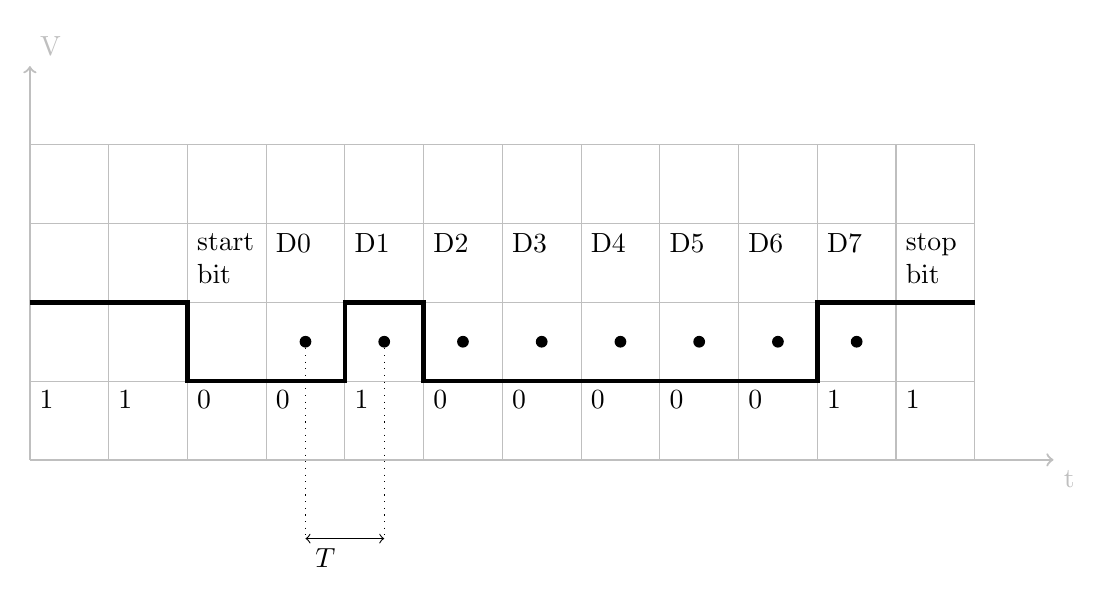
\begin{tikzpicture}
      \draw[lightgray] (0, 0) grid (12, 4);
      \draw[lightgray, thick, ->] (0, 0) -- (13, 0) node[anchor=north west] {t};
      \draw[lightgray, thick, ->] (0, 0) -- (0,  5) node[anchor=south west] {V};
      \draw[ultra thick, black] (0,  2) -- (2,   2)
      %% 0 (start bit)
      -- (2,   1) -- (3,   1)
      %% 0
      -- (4,   1)
      %% 1
      -- (4,   2) -- (5,   2)
      %% 0 x 5
      -- (5,   1) -- (10,   1)
      %% 1
      -- (10,   2)
      -- (11,   2)
      %% 1 (stop bits)
      -- (12,   2);
      %% Draw digits.
      \draw[black]
      (0,  1) node[anchor=north west] {1}
      (1,  1) node[anchor=north west] {1}
      (2,  1) node[anchor=north west] {0}
      (3,  1) node[anchor=north west] {0}
      (4,  1) node[anchor=north west] {1}
      (5,  1) node[anchor=north west] {0}
      (6,  1) node[anchor=north west] {0}
      (7,  1) node[anchor=north west] {0}
      (8,  1) node[anchor=north west] {0}
      (9,  1) node[anchor=north west] {0}
      (10, 1) node[anchor=north west] {1}
      (11, 1) node[anchor=north west] {1};
      %% Draw comments.
      \draw[black]
      (2,  3) node[anchor=north west, text width=1cm] {start bit}
      (11, 3) node[anchor=north west, text width=1cm] {stop bit};
      %% Draw bits.
      \draw[black]
      (3,  3) node[anchor=north west] {D0}
      (4,  3) node[anchor=north west] {D1}
      (5,  3) node[anchor=north west] {D2}
      (6,  3) node[anchor=north west] {D3}
      (7,  3) node[anchor=north west] {D4}
      (8,  3) node[anchor=north west] {D5}
      (9,  3) node[anchor=north west] {D6}
      (10, 3) node[anchor=north west] {D7};
      \foreach \x in {3.5, 4.5, 5.5, 6.5, 7.5, 8.5, 9.5, 10.5} {
        \node at (\x, 1.5)[circle,fill,inner sep=1.5pt]{};
      };
      \draw[black, dotted] (3.5, 1.5) -- (3.5, -1);
      \draw[black, dotted] (4.5, 1.5) -- (4.5, -1);
      \draw[<->, black]
      (3.5, -1) node[anchor=north west, text width=1cm] {$T$}
      -- (4.5, -1);
    \end{tikzpicture}
    \caption{\figureCaption}
    \label{fig:communication-serial-port-diagram}
  \end{figure}
}
